\documentclass[border=8pt,tikz]{standalone}
\usepackage[T1]{fontenc}
\usepackage{mathpazo}
\usepackage{xcolor}
\definecolor{clinteal}{RGB}{0,119,182}
\definecolor{clinred}{RGB}{213,94,0}
\definecolor{clinamber}{RGB}{230,159,0}
\definecolor{clingreen}{RGB}{0,158,115}
\usepackage{tikz}
\usetikzlibrary{shapes.geometric, arrows.meta, positioning, fit, calc, backgrounds}

\begin{document}
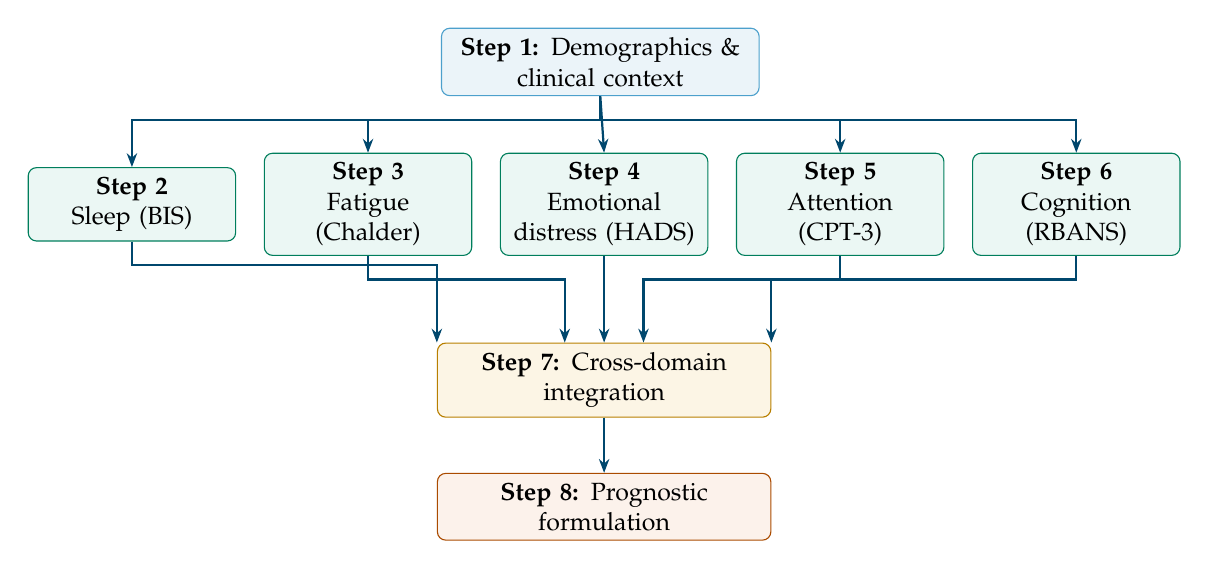
\begin{tikzpicture}[
    node distance=0.6cm and 0.35cm,
    ctxbox/.style={rectangle, rounded corners=3pt, draw=clinteal!70, fill=clinteal!8,
                   minimum height=0.8cm, text width=3.8cm, align=center, font=\small},
    dombox/.style={rectangle, rounded corners=3pt, draw=clingreen!80!black, fill=clingreen!8,
                   minimum height=0.8cm, text width=2.4cm, align=center, font=\small},
    intbox/.style={rectangle, rounded corners=3pt, draw=clinamber!80!black, fill=clinamber!10,
                   minimum height=0.8cm, text width=4.0cm, align=center, font=\small},
    progbox/.style={rectangle, rounded corners=3pt, draw=clinred!80!black, fill=clinred!8,
                    minimum height=0.8cm, text width=4.0cm, align=center, font=\small},
    arr/.style={-{Stealth[length=5pt]}, thick, clinteal!60!black},
]

\node[ctxbox] (s1) {\textbf{Step 1:} Demographics \&\\clinical context};

\node[dombox, below left=0.9cm and 2.6cm of s1] (s2) {\textbf{Step 2}\\Sleep (BIS)};
\node[dombox, right=0.35cm of s2] (s3) {\textbf{Step 3}\\Fatigue (Chalder)};
\node[dombox, right=0.35cm of s3] (s4) {\textbf{Step 4}\\Emotional distress (HADS)};
\node[dombox, right=0.35cm of s4] (s5) {\textbf{Step 5}\\Attention (CPT-3)};
\node[dombox, right=0.35cm of s5] (s6) {\textbf{Step 6}\\Cognition (RBANS)};

\node[intbox, below=1.1cm of s4] (s7) {\textbf{Step 7:} Cross-domain\\integration};

\node[progbox, below=0.7cm of s7] (s8) {\textbf{Step 8:} Prognostic\\formulation};

\draw[arr] (s1.south) -- ++(0,-0.3) -| (s2.north);
\draw[arr] (s1.south) -- ++(0,-0.3) -| (s3.north);
\draw[arr] (s1.south) -- (s4.north);
\draw[arr] (s1.south) -- ++(0,-0.3) -| (s5.north);
\draw[arr] (s1.south) -- ++(0,-0.3) -| (s6.north);

\draw[arr] (s2.south) |- ++(0,-0.3) -| (s7.north west);
\draw[arr] (s3.south) |- ++(0,-0.3) -| ([xshift=-0.5cm]s7.north);
\draw[arr] (s4.south) -- (s7.north);
\draw[arr] (s5.south) |- ++(0,-0.3) -| ([xshift=0.5cm]s7.north);
\draw[arr] (s6.south) |- ++(0,-0.3) -| (s7.north east);

\draw[arr] (s7.south) -- (s8.north);

\end{tikzpicture}
\end{document}
